\documentclass[a4paper, 12pt]{article}
\usepackage[utf8]{inputenc}
\usepackage{palatino}
\usepackage[breaklinks=true]{hyperref}
\usepackage{graphicx}
\usepackage{cprotect}
\usepackage{caption}
\usepackage[left=3cm, right=2cm, top=3cm, bottom=2cm]{geometry}
\geometry{a4paper}
\usepackage{fancyhdr}
\usepackage[brazilian]{babel}
\usepackage{siunitx}
\usepackage{subcaption}
\sisetup{detect-all}
\usepackage{float}
\usepackage{ragged2e}
\pagestyle{fancy}
\renewcommand{\headrulewidth}{0pt} 
\lhead{}\chead{}\rhead{}
\lfoot{}\cfoot{\thepage}\rfoot{}
\graphicspath{{figuras/}}
\usepackage{amsfonts}
\usepackage{mathtools}
\usepackage{cleveref}
\usepackage{spverbatim}
\usepackage[framed,numbered,autolinebreaks,useliterate]{mcode}
\setlength{\parskip}{1em}
\usepackage{xspace}
\usepackage{amsmath}
\usepackage{gensymb}
\usepackage{booktabs}
\usepackage{minted}
\usepackage{listings}
\usepackage{bm}
\usepackage{indentfirst}
\usepackage{algorithm}
\usepackage{algpseudocode, lipsum}
\lstset{
    literate={~} {$\sim$}{1}
}
\usepackage[shortlabels]{enumitem}

\newcommand{\MATLAB}{\textsc{Matlab}\xspace}
\newcommand{\SIMULINK}{\textsc{Simulink}\xspace}
\newcommand{\pspice}{\textsc{PSpice}\xspace}
\newcommand{\Python}{\textsc{Python}\xspace}
\newcommand{\tinkercad}{\textsc{TinkerCad}\xspace}
\newcommand{\arduino}{\textsc{Arduino}\xspace}
\newcommand{\sen}{\hspace{2pt}\mathrm{sen}}
\newcommand{\counts}{\textit{counts}\xspace}
\newcommand{\FT}{\text{F.T.}}
\newcommand{\zeros}{\text{Zeros}}
\newcommand{\polos}{\text{Polos}}
\newcommand{\software}{\textit{software}\xspace}
\newcommand{\hardware}{\textit{hardware}\xspace}
\newcommand{\fitness}{\textit{fitness}\xspace}
\newcommand{\fitsha}{\textit{fitness sharing}\xspace}


\newenvironment{brprocess}[1][]
  {\begin{algorithm}[#1]
     \selectlanguage{brazilian}%
     \floatname{algorithm}{Processo}%
     \renewcommand{\algorithmicif}{\textbf{se}}%
     \renewcommand{\algorithmicfor}{\textbf{para}}%
     \renewcommand{\algorithmicdo}{\textbf{faça}}%
     \renewcommand{\algorithmicthen}{\textbf{faça}}%
     \renewcommand{\algorithmicend}{\textbf{fim}}%
     \renewcommand{\algorithmicwhile}{\textbf{enquanto}}%
     \renewcommand{\algorithmicelse}{\textbf{caso contrário}}%
     % Set other language requirements
  }
  {\end{algorithm}}

  \newenvironment{bralgorithm}[1][]
  {\begin{algorithm}[#1]
     \selectlanguage{brazilian}%
     \floatname{algorithm}{Algoritmo}%
     \renewcommand{\algorithmicif}{\textbf{se}}%
     \renewcommand{\algorithmicfor}{\textbf{para}}%
     \renewcommand{\algorithmicdo}{\textbf{faça}}%
     \renewcommand{\algorithmicthen}{\textbf{faça}}%
     \renewcommand{\algorithmicend}{\textbf{fim}}%
     \renewcommand{\algorithmicwhile}{\textbf{enquanto}}%
     \renewcommand{\algorithmicelse}{\textbf{caso contrário}}%
     % Set other language requirements
  }
  {\end{algorithm}}

\begin{document}
\begin{titlepage}
\newcommand{\HRule}{\rule{\linewidth}{0.5mm}}
	
\centering

\includegraphics[width=0.15\textwidth]{logo-unicamp.pdf}\\[0.5cm]	
\textsc{\Large Universidade Estadual de Campinas}\\[2.0cm]
\textsc{\large Faculdade de Engenharia Elétrica e de Computação}\\[0.5cm]
	
\textsc{IA707/EG507 - Computação Evolutiva}\\[2.5cm]
	
{\LARGE \bfseries EFC II}\\[3.5cm]

\begin{minipage}[t]{0.4\textwidth}
	\begin{flushleft}
    \textit{Alunos}\\
    João Pedro O. Pagnan - 199727
	\end{flushleft}
\end{minipage}
~
\begin{minipage}[t]{0.4\textwidth}
	\begin{flushright}
		\textit{Professor}\\
		Levy Boccato
	\end{flushright}
\end{minipage}\\[4.5cm]

{Campinas, \today}

\vfill\vfill\vfill\vfill\vfill

\includegraphics[width=0.2\textwidth]{logo-feec.png}\\[0.5cm]
\vfill

\end{titlepage}

\justify

Neste exercício, vamos abordar o problema de otimização de função multimodal, com o auxílio de um algoritmo genético (GA, do inglês \textit{genetic algorithm}). Iremos considerar a função contínua
$$f (x, y) = x \cdot \sen(4\pi \cdot x) - y \cdot \sen(4\pi \cdot y + \pi) + 1,$$
onde $x, y \in [-1, 2]$ e desejamos determinar o ponto $(x^{*} , y^{*})$ que maximize a função $f(\cdot )$.
\begin{figure}[H]
    \centering
    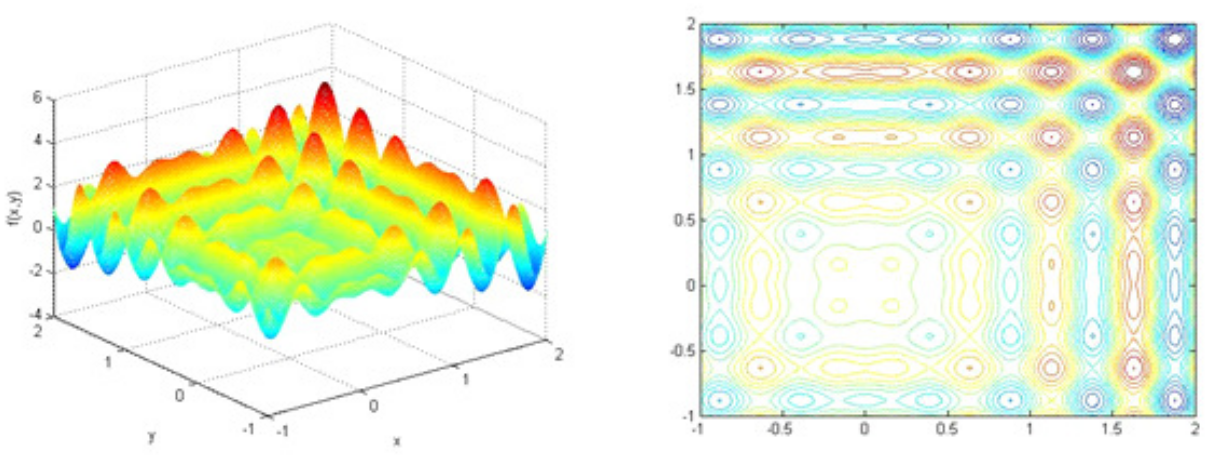
\includegraphics[width=0.8\textwidth]{figuras/grafico-funcao.png}
    \caption{Visualização da superfície e das curvas de nível da função $f (x, y)$.}
    \label{fig:grafico-funcao}
\end{figure}

\textbf{(a) Proponha um algoritmo genético (AG) para encontrar o máximo global de $f(x, y)$. Descreva todos os elementos que o compõem – codificação, função de \fitness, operadores, etc. — e justifique suas escolhas.}

O algoritmo genético para encontrar o máximo global de $f(x, y)$ será composto pelo seguinte passo a passo:
\begin{enumerate}
    \item Gerar a população inicial com $N$ indivíduos representados pela codificação adotada;
    \item Calcular o \fitness para cada indivíduo da população inicial;
    \item Aplicar o operador de seleção para selecionar dois indivíduos baseado em seus \textit{fitness};
    \item Aplicar o operador de recombinação para gerar dois descendentes;
    \item Aplicar o operador de mutação nos descendentes para que os respectivos cromossomos tenham uma probabilidade $p_m$ de serem mutados;
    \item Caso o número total de indivíduos e descendentes for menor que $2N$, repetir do passo 3 ao 5;
    \item Calcular o \fitness dos descendentes;
    \item Eliminar os $N$ indivíduos de menor \fitness;
    \item Repetir do passo 3 ao 8 até o critério de parada ser atingido.
\end{enumerate}

No caso, a codificação adotada escolhida foi a \textbf{codificação real}, em que cada indivíduo, ou solução, é representada por um vetor bidimensional cujos elementos são números reais, isto é, sendo $\bm{z}$ um indivíduo da população:
\begin{equation}
    \bm{z} = \left[x, y \right],
\end{equation}
com $x,y \in [-1, 2]$.

A \textbf{geração da população inicial} será da forma indicada no processo \ref{alg:pop-inicial}, sendo $N$ o tamanho da população.
\begin{brprocess}[!ht]
    \textbf{Paramêtros}: Tamanho da população desejada\\
    \textbf{Saída}: População gerada
    \cprotect\caption{Geração aleatória da população inicial (\verb|gerar_pop(N)|)}
    \begin{algorithmic}
    \State população $\gets [\;]$
    \State $i\gets 0$
    \While{$i < N$}
        \State cromossomo $\gets [\;]$
        \State $j \gets 0$
        \While{$j < 2$}
            \State gene $\gets$ alelo $\in [-1, 2]]$
            \State cromossomo $[j] \gets$ gene
            \State $j \gets j + 1$
        \EndWhile
        \State \textit{fitness} $\gets 0$
        \State população $[i] \gets$ [cromossomo, \textit{fitness}]
        \State $i \gets i + 1$
    \EndWhile
    \State \textbf{retorna} população
    \end{algorithmic}
    \label{alg:pop-inicial}
\end{brprocess}

A função de avaliação, ou \fitness, adotada é a própria função que deseja-se maximizar. Desta forma, ela é dada por:
\begin{equation}\label{eq:fitness}
    \phi(\bm{z}) = \phi(x, y) = x \cdot \sen(4\pi \cdot x) - y \cdot \sen(4\pi \cdot y + \pi) + 1
\end{equation}

\textbf{(b) Para cada uma de 5 execuções independentes do AG, apresente as curvas de \fitness médio e de \fitness do melhor indivíduo em função do número de gerações. Mostre também, tendo por pano de fundo as curvas de nível da função $f(x, y)$, a distribuição dos indivíduos da população final em cada execução. Com base nesse conjunto de gráficos, busque analisar o algoritmo em termos de sua eficiência de busca e manutenção de diversidade.}

\textbf{(c) Implemente agora o método de \fitsha. Comente as escolhas feitas para os valores dos parâmetros (e.g., $\sigma_s$) e de operadores (caso alguma modificação em relação ao item (b) tenha sido necessária). Repita o procedimento do item (b) para analisar o comportamento do \fitsha.}

\textbf{(d) Introduza, por fim, o esquema de restrição de cruzamento (seguindo o espírito da abordagem de especiação) proposto por \cite{deb1989genetic} Analise o impacto da inserção deste mecanismo na evolução da população e, em última análise, no desempenho do algoritmo.}

\clearpage

\bibliographystyle{ieeetr}

\bibliography{bib}

\pdfinfo{
   /Title  (IA707 - EFC II - 199727)
}
 \end{document}